% !TeX root = Bericht.tex
% !TeX spellcheck = de_DE 
\section{Appendix}

\begin{figure}[H]
	\centering
	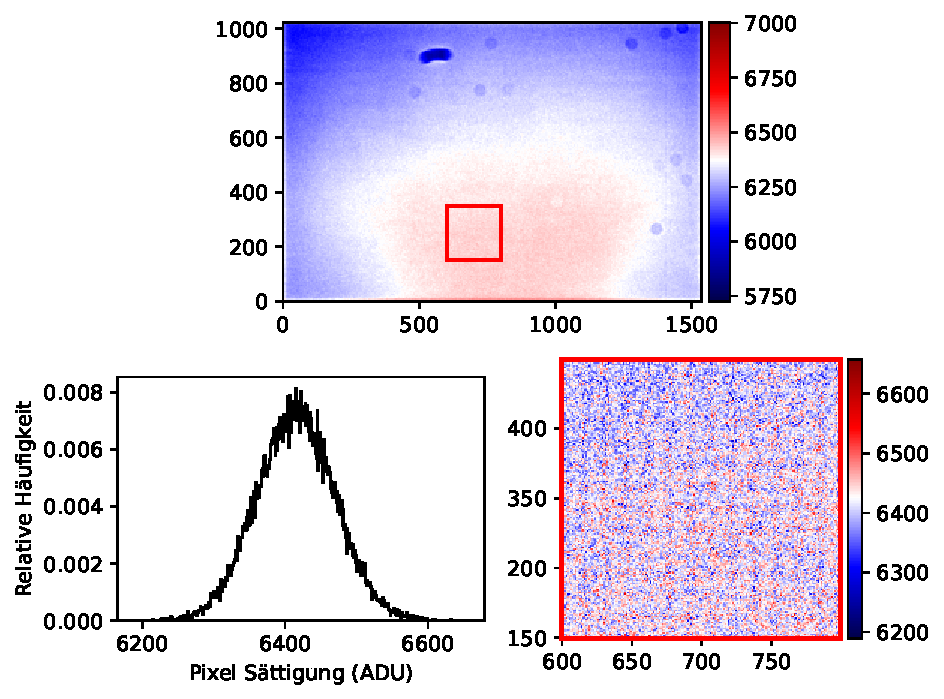
\includegraphics[width=\linewidth]{ex2_Green}
	\caption{Zu sehen ist oben das gesamte Flatfield-Frame des CCD für die grüne Folie, rechts unten ist auf das rote Quadrat gezoomt. Links unten ist ein Histogramm der  Pixel Sättigung gezeigt. }
	\label{blau_aufgabe3}
\end{figure}
\begin{figure}[H]
	\centering
	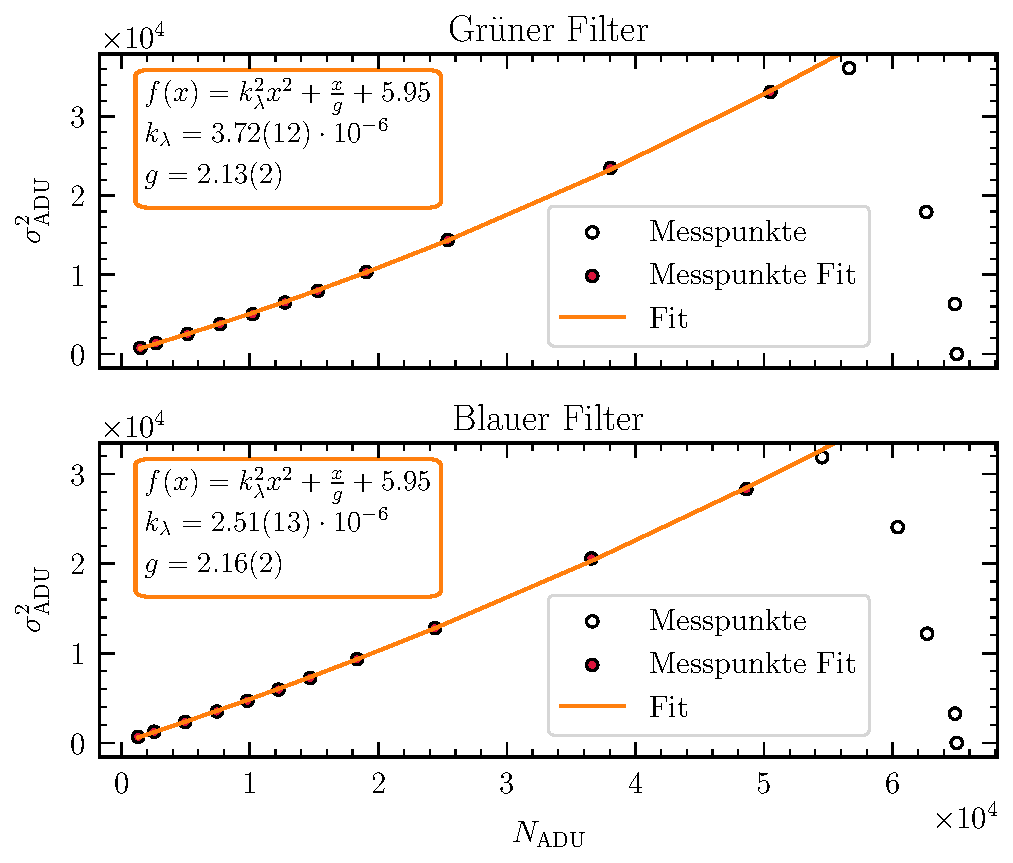
\includegraphics{ex5_2}
	\caption{Zu sehen ist die quadrierte Standardabweichung in ADU abhängig der Signastärke in ADU für die grüne und die blaue Folie. Ebenso sind Fitfunktionen an die Daten angepasst worden. Bei dieser Fitfunktion wurde der Nulldurchgang der y-Achse als gegeben angenommen (Berechnet in Aufgabe 2).}
	\label{fig:ex5_2}
\end{figure}